%======================================================================
\section{Is IHS for MaxSAT Equivalent to Dantzig--Wolfe? A Worked Example and a Counterexample}
\label{sec:part2}
%======================================================================

%----------------------------------------------------------------------
\subsection{The Claim, Stated Precisely}
\label{sec:claim}
%----------------------------------------------------------------------

\cref{sec:part1} argued that Implicit Hitting Set (IHS) MaxSAT solvers
implement Dantzig--Wolfe (DW) decomposition, viewed through LP duality. Here we
test that claim concretely. We first state the equivalence precisely and prove
the row/column duality that underlies it. We then work a small instance step by
step, running IHS and DW column generation side by side and observing that they
generate the same cores, in the same order, with the same bounds, and terminate
with the same value. Finally we exhibit a counterexample: a three-clause
instance on which DW column generation terminates at the value $3/2$ while
IHS---and the true MaxSAT optimum---is $2$. The resolution is sharp: \textbf{IHS
with an LP master is exactly DW on the dual core-packing LP, but the IHS used in
practice solves the master as an integer program, which is strictly stronger than
DW and breaks literal equivalence.} The equivalence is therefore real but
conditional, and the condition (LP vs.\ integer master) is exactly the
integrality gap of the hitting-set polytope.

Fix a weighted partial MaxSAT instance $\langle \mathcal{H}, \mathcal{S}, w
\rangle$ with soft clauses $\mathcal{S} = \{s_1,\dots,s_m\}$ and weights
$w_i = w(s_i) > 0$. For $y \in \{0,1\}^m$ read $y_i = 1$ as ``$s_i$ is
falsified.'' Let $\mathcal{K}$ be the (exponential) family of all cores
$\kappa \subseteq \mathcal{S}$, i.e.\ subsets with $\mathcal{H} \cup \kappa$
unsatisfiable. MaxSAT is the \emph{minimum-cost hitting set} over $\mathcal{K}$:
\begin{align}
(\mathrm{IP})\qquad
z^\star = \min \;\; & \textstyle\sum_{i} w_i\, y_i \notag\\
\text{s.t.} \;\; & \textstyle\sum_{s_i \in \kappa} y_i \ge 1 \quad \forall \kappa \in \mathcal{K}, \label{eq:hit}\\
& y_i \in \{0,1\}. \notag
\end{align}
Its LP relaxation replaces $y_i \in \{0,1\}$ by $y_i \ge 0$ (the upper bound
$y_i \le 1$ is slack at the optimum of a minimization). Call its value
$z^\star_{\mathrm{LP}}$. The LP \emph{dual} assigns a variable
$\lambda_\kappa \ge 0$ to each core and is a \emph{fractional core packing}:
\begin{align}
(\mathrm{D})\qquad
z^\star_{\mathrm{LP}} = \max \;\; & \textstyle\sum_{\kappa} \lambda_\kappa \notag\\
\text{s.t.} \;\; & \textstyle\sum_{\kappa \ni s_i} \lambda_\kappa \le w_i \quad \forall i = 1,\dots,m, \label{eq:pack}\\
& \lambda_\kappa \ge 0. \notag
\end{align}

\paragraph{What ``Dantzig--Wolfe'' means here.} Dantzig--Wolfe decomposition
reformulates a structured LP so that its variables are indexed by an exponential
family (the extreme points of a subproblem polyhedron), and solves the
reformulation by \emph{column generation}: maintain a \emph{restricted master}
with only a working subset of columns, read off dual prices, and call a
\emph{pricing subproblem} that either returns a new column of negative reduced
cost or certifies optimality. We take ``IHS is DW'' to mean precisely:
\emph{IHS is column generation applied to the dual packing LP}~\eqref{eq:pack},
where each core is a column.

\paragraph{What IHS does.} IHS keeps a working set $\mathcal{K}_t \subseteq
\mathcal{K}$ of \emph{discovered} cores, solves the \emph{restricted} master
\eqref{eq:hit} over $\mathcal{K}_t$ to get $H_t^\star$ (the set of $s_i$ with
$y_i = 1$), then calls a SAT oracle on $\mathcal{H} \cup (\mathcal{S} \setminus
H_t^\star)$. If SAT, $H_t^\star$ is an achievable correction set and, being a
minimum hitting set of all known cores, is optimal: stop. If UNSAT, the oracle
returns a core $\kappa$ \emph{not hit} by $H_t^\star$; add it and repeat. The
only design choice we vary below is whether the master \eqref{eq:hit} is solved
as an integer program (\textbf{IHS-IP}, the practical solver, e.g.\ MaxHS) or as
its LP relaxation (\textbf{IHS-LP}).

%----------------------------------------------------------------------
\subsection{The Exact Equivalence (LP Master)}
\label{sec:equiv}
%----------------------------------------------------------------------

The bridge is the textbook fact that \emph{generating rows of an LP is
generating columns of its dual}. We state it for our setting.

\begin{lemma}[Row generation $=$ column generation across duality]
\label[lemma]{lem:rowcol}
Let $\mathcal{K}_t \subseteq \mathcal{K}$. The restricted primal LP---
\eqref{eq:hit} relaxed to $y\ge0$ and limited to cores in $\mathcal{K}_t$---and
the restricted dual---\eqref{eq:pack} limited to the columns $\{\lambda_\kappa :
\kappa \in \mathcal{K}_t\}$---are an LP dual pair. Consequently:
\begin{enumerate}
\item[(i)] they have equal optimal value $v_t$, and the primal optimum $y^{(t)}$
is the vector of dual prices of the restricted dual;
\item[(ii)] a core $\kappa \in \mathcal{K}\setminus\mathcal{K}_t$ is
\emph{violated} by $y^{(t)}$ in the primal, i.e.\ $\sum_{s_i \in \kappa}
y^{(t)}_i < 1$, \emph{iff} the column $\lambda_\kappa$ has \emph{strictly
positive reduced cost} $\bar c_\kappa = 1 - \sum_{s_i\in\kappa} y^{(t)}_i$ in
the dual;
\item[(iii)] adding $\kappa$ to $\mathcal{K}_t$ adds one row to the primal and,
identically, one column to the dual.
\end{enumerate}
\end{lemma}

\begin{proof}
The dual of $\min\{w^\top y : A_t y \ge \mathbf 1,\ y \ge 0\}$ is $\max\{\mathbf
1^\top\lambda : A_t^\top \lambda \le w,\ \lambda \ge 0\}$, where $A_t$ is the
core-incidence matrix whose rows are the cores in $\mathcal{K}_t$. The first is
the restricted primal, the second the restricted dual; (i) is strong LP duality
and complementary reading of the simplex multipliers. For (ii), the dual
objective coefficient of $\lambda_\kappa$ is $1$ and its column in $A_t^\top$ is
the incidence vector of $\kappa$. Since the dual is a \emph{maximization}, we
adopt the standard convention that an entering column is one with
\emph{strictly positive} reduced cost (objective coefficient minus the
dual-price contribution). With prices $y^{(t)}$ the reduced cost is
$\bar c_\kappa = 1 - \sum_{s_i \in \kappa} y^{(t)}_i$, positive exactly when
$\kappa$ is under-hit. (iii) is immediate from the transpose relationship.
\end{proof}

\begin{proposition}[IHS-LP is Dantzig--Wolfe on the dual]
\label[proposition]{prop:equiv}
Run IHS-LP and column generation on the dual packing
LP~\eqref{eq:pack} from the same initial working set, with the SAT oracle as the
pricing routine, and assume:
\begin{itemize}
\item[(a)] both runs use a \emph{deterministic} LP solver that, on inputs with
the same constraint matrix, returns the same basic optimum (so degeneracy is
broken identically on both sides); and
\item[(b)] a common tie-breaking rule selects, among multiple violated /
under-priced cores, the one the oracle returns.
\end{itemize}
Then at every iteration the two algorithms hold the same working set
$\mathcal{K}_t$, the same master value $v_t$, and---given (b)---generate the
\emph{same} core. Both terminate with value $z^\star_{\mathrm{LP}}$.
\end{proposition}

\begin{proof}
Induction on $t$. The master values agree by \cref{lem:rowcol}(i). At the
pricing step, IHS-LP seeks a core violated by $y^{(t)}$; column generation seeks
a column of positive reduced cost; by \cref{lem:rowcol}(ii) these are the
\emph{same set of candidate cores}, so under (b) a shared oracle returns the
same $\kappa$, and by (iii) the two working sets stay equal. Termination is
simultaneous: ``no violated core'' $=$ ``no positive-reduced-cost column,'' and
the common value is the full LP optimum $z^\star_{\mathrm{LP}}$ because all
violated cores have been priced out.
\end{proof}

\begin{remark}[Degeneracy]
\label[remark]{rem:degeneracy}
Hypothesis (a) is genuinely needed: the restricted LP can have multiple optima
(e.g.\ on $K_3$ (\cref{sec:counter}) after the single core $\kappa_{12}$, both
$y=(1,0,0)$ and $y=(0,1,0)$ are optimal; after a second core the optimum
becomes unique again---the clause shared by the two cores),
and two solvers returning different bases will ask the SAT oracle different
pricing questions and may extract different cores. The master \emph{value}
still agrees in lockstep---only the trajectory of generated cores can fork.
This is the same degeneracy that motivates dual-stabilization techniques
(\cref{sec:techniques}).
\end{remark}

\begin{remark}[Fractional pricing is not one SAT call]
\label[remark]{rem:fracpricing}
\Cref{prop:equiv} equips IHS-LP with an oracle that, given the
\emph{fractional} prices $y^{(t)}$, finds a core $\kappa$ with
$\sum_{s_i \in \kappa} y^{(t)}_i < 1$ or certifies that none exists. When
$y^{(t)}$ is integral, this is exactly one SAT call on
$\mathcal{H} \cup (\mathcal{S} \setminus H_t^\star)$---the standard IHS
oracle---and that is the case throughout the $P_4$ trace of
\cref{sec:worked}. For genuinely fractional $y^{(t)}$, however, separation
asks for an unsatisfiable subset of fractional weight below~$1$. This is a
\emph{weighted-MUS-type optimization} (find $\kappa$ minimizing $\sum_{s_i \in \kappa} y_i^{(t)}$)
that no single SAT call implements. Thus IHS-LP, unlike IHS-IP, is \emph{not}
implementable with the unmodified IHS oracle; this is a second, independent
sense in which practical IHS departs from textbook column generation.
Conveniently, the integer master of practical IHS guarantees integral prices,
which is precisely what lets a plain SAT call serve as the separation routine
(cf.\ \cref{sec:subtle}, point~2). \Cref{sec:cg-gap} develops outer-loop
approximations to exactly this fractional pricing problem.
\end{remark}

\cref{prop:equiv} is the precise, defensible content of the slogan
``IHS is Dantzig--Wolfe in the dual.'' Note three things it does \emph{not} say,
which we revisit in \cref{sec:subtle}: it concerns the \emph{LP} master; the
oracle is used as a \emph{separation} oracle (find \emph{some} violated core),
not a true DW pricing oracle (find the \emph{most} negative reduced cost); and
the dual~\eqref{eq:pack} has no convexity row $\sum_\kappa \lambda_\kappa = 1$,
so it is column generation in general, of which DW is the special case where
columns are extreme points of a fixed polyhedron.

%----------------------------------------------------------------------
\subsection{A Step-by-Step Example Where They Coincide}
\label{sec:worked}
%----------------------------------------------------------------------

We now make \cref{prop:equiv} concrete on an instance whose
hitting-set polytope is \emph{integral}, so IHS-IP, IHS-LP, and DW all agree.

\subsubsection{The Instance \texorpdfstring{$P_4$}{P4}}

Four soft \emph{unit} clauses with unit weight,
\[
s_1=(x_1),\quad s_2=(x_2),\quad s_3=(x_3),\quad s_4=(x_4),\qquad w_i = 1,
\]
and three hard clauses forbidding adjacent pairs from being true together,
\[
\mathcal{H} = \{(\bar x_1 \vee \bar x_2),\ (\bar x_2 \vee \bar x_3),\ (\bar x_3 \vee \bar x_4)\}.
\]
Setting $x_i$ true falsifies nothing in $\mathcal{H}$ by itself, so each
singleton soft set is satisfiable; a pair $\{s_i,s_j\}$ is unsatisfiable with
$\mathcal{H}$ \emph{iff} $\{i,j\}$ is an edge of the path $1{-}2{-}3{-}4$. One
checks that every $3$-subset of $\{1,2,3,4\}$ contains an edge, so the
\textbf{minimal cores are exactly the three edges} (see \cref{fig:p4-k3},
left):
\[
\kappa_a = \{s_1,s_2\},\qquad \kappa_b = \{s_2,s_3\},\qquad \kappa_c = \{s_3,s_4\}.
\]
Hitting all edges is the minimum \emph{vertex cover} of the path; the path is
bipartite, so by K\H{o}nig's theorem the LP relaxation is integral and
$z^\star = z^\star_{\mathrm{LP}} = 2$ (e.g.\ cover $\{s_2,s_3\}$; equivalently
the MaxSAT optimum keeps the independent set $\{x_1,x_3\}$ true and falsifies
two clauses).

\subsubsection{Running IHS-IP and DW in Lockstep}

We let the SAT oracle, when several cores are unhit, return them in the fixed
order $\kappa_a, \kappa_b, \kappa_c$ (any common rule works, fulfilling Hypothesis (b)
of \cref{prop:equiv} to ensure both algorithms trace the exact same path). \cref{tab:trace-p4}
traces both algorithms. For DW we report the dual prices $y^{(t)}$ (the
restricted-primal optimum) used by pricing, and the dual master value; for
IHS we report the integer hitting set $H_t^\star$ and the lower bound. Recall
the pricing test from \cref{lem:rowcol}(ii): a core $\kappa$ is improving
iff $\sum_{s_i\in\kappa} y^{(t)}_i < 1$.

\begin{table}[htbp]
\centering
\small
\begin{tabular}{c l l c l}
\toprule
$t$ & Working set $\mathcal{K}_t$ & IHS-IP master $H_t^\star$ (LB) & DW prices $y^{(t)}$ & Pricing $\to$ new core \\
\midrule
$1$ & $\emptyset$ & $\emptyset$ \;(LB $0$) & $(0,0,0,0)$ & $\kappa_a$: $0<1$ \;$\Rightarrow$ add $\kappa_a$\\
$2$ & $\{\kappa_a\}$ & $\{s_1\}$ \;(LB $1$) & $(1,0,0,0)$ & $\kappa_b$: $y_2{+}y_3{=}0$ \;$\Rightarrow$ add $\kappa_b$\\
$3$ & $\{\kappa_a,\kappa_b\}$ & $\{s_2\}$ \;(LB $1$) & $(0,1,0,0)$ & $\kappa_c$: $y_3{+}y_4{=}0$ \;$\Rightarrow$ add $\kappa_c$\\
$4$ & $\{\kappa_a,\kappa_b,\kappa_c\}$ & $\{s_2,s_3\}$ \;(LB $2$) & $(0,1,1,0)$ & all cores hit \;$\Rightarrow$ \textbf{stop} \\
\bottomrule
\end{tabular}
\caption{IHS-IP and DW column generation on $P_4$, in lockstep. The master
value (LB) and the dual master value coincide at every step ($0,1,1,2$); the
same cores are generated in the same order; both stop at $t=4$ with value $2$.}
\label{tab:trace-p4}
\end{table}

\paragraph{Reading the steps.}
\begin{itemize}
\item \textbf{$t=1$.} No cores known. Master is empty $\Rightarrow H^\star =
\emptyset$, prices $y=0$. The SAT oracle on $\mathcal{H}\cup\{x_1,x_2,x_3,x_4\}$
is UNSAT (all-true violates every hard clause) and returns $\kappa_a$. In DW,
$\bar c_{\kappa_a} = 1 - 0 = 1 > 0$: the identical column.
\item \textbf{$t=2$.} Master $\min \sum y_i$ s.t.\ $y_1+y_2 \ge 1$ gives
$H^\star=\{s_1\}$ and dual prices $y=(1,0,0,0)$, value $1$ on both sides.
SAT on $\mathcal{H}\cup\{x_2,x_3,x_4\}$ is UNSAT, oracle returns $\kappa_b$
(unhit: $y_2+y_3 = 0 < 1$).
\item \textbf{$t=3$.} Master s.t.\ $y_1+y_2\ge1,\ y_2+y_3\ge1$ gives the cheaper
cover $H^\star=\{s_2\}$, prices $y=(0,1,0,0)$, value $1$. SAT on
$\mathcal{H}\cup\{x_1,x_3,x_4\}$ is UNSAT, oracle returns $\kappa_c$
($y_3+y_4 = 0 < 1$).
\item \textbf{$t=4$.} Master s.t.\ all three constraints gives $H^\star=\{s_2,s_3\}$,
value $2$; dually $\lambda_{\kappa_a}=\lambda_{\kappa_c}=1,\lambda_{\kappa_b}=0$
packs to $2$. With $y=(0,1,1,0)$ every core is hit ($\kappa_a$: $y_2$; $\kappa_b$:
$y_2,y_3$; $\kappa_c$: $y_3$), so DW prices out and IHS's SAT call on
$\mathcal{H}\cup\{x_1,x_4\}$ succeeds ($x_1,x_4$ true, $x_2,x_3$ false). Both
return $\mathbf 2$.
\end{itemize}

On $P_4$ the two algorithms are not merely structurally analogous---they are
\emph{the same run} of one algorithm read in two dual coordinate systems,
exactly as \cref{prop:equiv} predicts. The reason it works without
caveats is that $z^\star = z^\star_{\mathrm{LP}}$: the integer master never
disagrees with the LP master.

%----------------------------------------------------------------------
\subsection{A Counterexample: The Triangle of Cores}
\label{sec:counter}
%----------------------------------------------------------------------

Equivalence is conditional on that last clause. We now remove the condition.
\Cref{fig:p4-k3} previews the contrast that this subsection develops: $P_4$
is bipartite, the hitting-set LP is integral, and all three algorithms agree;
$K_3$ is an odd cycle, the LP relaxation is strictly fractional, and the
integer master used by practical IHS strictly dominates pure Dantzig--Wolfe.

\begin{figure}[t]
\centering
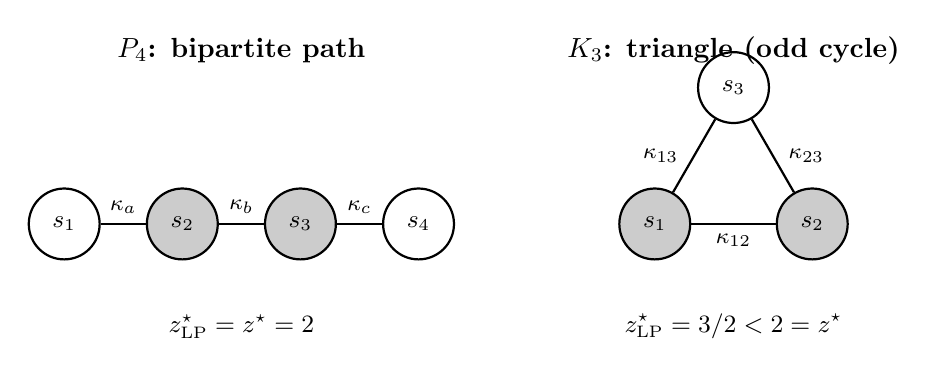
\begin{tikzpicture}[
    every node/.style={font=\small},
    vert/.style={circle, draw, thick, minimum size=9mm, inner sep=1pt},
    covered/.style={vert, fill=black!20},
    elbl/.style={font=\footnotesize},
    title/.style={font=\bfseries},
]
% Left panel: P_4
\begin{scope}
  \node[title] at (2.25,2.2) {$P_4$: bipartite path};
  \node[vert]    (a1) at (0,0)   {$s_1$};
  \node[covered] (a2) at (1.5,0) {$s_2$};
  \node[covered] (a3) at (3,0)   {$s_3$};
  \node[vert]    (a4) at (4.5,0) {$s_4$};
  \draw[thick] (a1) -- node[elbl, above] {$\kappa_a$} (a2);
  \draw[thick] (a2) -- node[elbl, above] {$\kappa_b$} (a3);
  \draw[thick] (a3) -- node[elbl, above] {$\kappa_c$} (a4);
  \node at (2.25,-1.3) {$z^\star_{\mathrm{LP}} = z^\star = 2$};
\end{scope}
% Right panel: K_3
\begin{scope}[xshift=7.5cm]
  \node[title] at (1,2.2) {$K_3$: triangle (odd cycle)};
  \node[covered] (b1) at (0,0)        {$s_1$};
  \node[covered] (b2) at (2,0)        {$s_2$};
  \node[vert]    (b3) at (1,1.732)    {$s_3$};
  \draw[thick] (b1) -- node[elbl, below]     {$\kappa_{12}$} (b2);
  \draw[thick] (b1) -- node[elbl, left=2pt]  {$\kappa_{13}$} (b3);
  \draw[thick] (b2) -- node[elbl, right=2pt] {$\kappa_{23}$} (b3);
  \node at (1,-1.3) {$z^\star_{\mathrm{LP}} = 3/2 < 2 = z^\star$};
\end{scope}
\end{tikzpicture}
\caption{The two instances as graphs whose vertices are soft clauses and
whose edges are the minimal cores. Shaded vertices give an optimal integer
hitting set $H^\star$. On the bipartite path $P_4$ (left) the LP relaxation
of the hitting-set polytope is integral, so IHS-IP, IHS-LP, and
Dantzig--Wolfe column generation all return the same value~$2$. On the
triangle $K_3$ (right) the LP optimum is $y_1 = y_2 = y_3 = \tfrac12$ with
value $3/2$, whereas any integer cover has size~$2$; the $4/3$
integrality gap is exactly where pure Dantzig--Wolfe (terminating at $3/2$)
and the integer-master IHS used in practice (returning $2$) part ways.}
\label{fig:p4-k3}
\end{figure}

\subsubsection{The Instance \texorpdfstring{$K_3$}{K3}}

Three soft unit clauses with unit weight and the ``at most one true'' hard
clauses,
\[
s_1=(x_1),\ s_2=(x_2),\ s_3=(x_3),\quad w_i=1,\qquad
\mathcal{H} = \{(\bar x_1\vee\bar x_2),\ (\bar x_1\vee\bar x_3),\ (\bar x_2\vee\bar x_3)\}.
\]
Each singleton is satisfiable; each pair is a minimal core, and the triple is
not minimal. The \textbf{minimal cores are the three pairs}
\[
\kappa_{12}=\{s_1,s_2\},\quad \kappa_{13}=\{s_1,s_3\},\quad \kappa_{23}=\{s_2,s_3\},
\]
forming a triangle $K_3$---an \emph{odd} cycle, hence non-bipartite, hence with
a fractional vertex-cover gap. For the true MaxSAT optimum, since at most one $x_i$ may be
true, at least two soft clauses must be falsified, and $z^\star = 2$.

\subsubsection{What DW Computes}
\label{sec:dwcomputes}

The full dual packing LP~\eqref{eq:pack} is
\[
\max\ \lambda_{12}+\lambda_{13}+\lambda_{23}
\quad\text{s.t.}\quad
\underbrace{\lambda_{12}+\lambda_{13}}_{s_1}\le1,\
\underbrace{\lambda_{12}+\lambda_{23}}_{s_2}\le1,\
\underbrace{\lambda_{13}+\lambda_{23}}_{s_3}\le1,\
\lambda\ge0.
\]
Summing the three constraints gives $2(\lambda_{12}+\lambda_{13}+\lambda_{23})
\le 3$, so the objective is at most $3/2$, attained at $\lambda_{12} =
\lambda_{13} = \lambda_{23} = \tfrac12$. Dually $y_1=y_2=y_3=\tfrac12$ is primal
optimal with cost $3/2$. Column generation reaches exactly this: after all three
cores are columns, the prices are $y=(\tfrac12,\tfrac12,\tfrac12)$, every core
has reduced cost $1 - (\tfrac12+\tfrac12) = 0$, no improving column exists, and
DW \textbf{terminates with value $\boldsymbol{3/2}$}. This is confirmed
empirically by the prototype \texttt{IHSSolver} in \texttt{src/ihs.py}, which
implements \cref{alg:ihs} with the master solved both as a 0/1 IP
(via PuLP/CBC) and as an LP relaxation, calling MiniSat-family assumption
SAT for the oracle. On the 3-clause WCNF encoding \texttt{src/wcnf/k3.wcnf}
the IP master returns cost $2$ (matching $z^\star$) while the LP master
value stabilizes at exactly $1.5$ (matching $z^\star_{\mathrm{LP}}$), so
both halves of \cref{tab:counter} are observed in a single run.

\subsubsection{What IHS Computes}
\label{sec:ihscomputes}

IHS generates the same three cores, but its master is the \emph{integer} hitting
set
\[
\min\ y_1+y_2+y_3 \quad\text{s.t.}\quad y_1+y_2\ge1,\ y_1+y_3\ge1,\ y_2+y_3\ge1,\ y\in\{0,1\}^3,
\]
whose optimum is $2$ (e.g.\ $H^\star=\{s_1,s_2\}$). The SAT oracle on
$\mathcal{H}\cup(\mathcal{S}\setminus H^\star)=\mathcal{H}\cup\{(x_3)\}$ succeeds
($x_3$ true, $x_1,x_2$ false), certifying a correction set of cost $2$. IHS
\textbf{terminates with value $\boldsymbol{2} = z^\star$}.

\begin{table}[htbp]
\centering
\small
\begin{tabular}{l c c c}
\toprule
& cores generated & terminal value & is it $z^\star=2$? \\
\midrule
DW / column generation on \eqref{eq:pack} & $\kappa_{12},\kappa_{13},\kappa_{23}$ & $3/2$ & \textbf{no} \\
IHS-LP (LP master) & $\kappa_{12},\kappa_{13},\kappa_{23}$ & $3/2$ & \textbf{no} \\
IHS-IP (integer master, real solvers) & $\kappa_{12},\kappa_{13},\kappa_{23}$ & $2$ & \textbf{yes} \\
\bottomrule
\end{tabular}
\caption{On the triangle $K_3$, DW and IHS-LP agree with each other (value
$3/2$) but disagree with IHS-IP and with the true optimum (value $2$). The gap
is the integrality gap $z^\star/z^\star_{\mathrm{LP}} = 4/3$ of the hitting-set
polytope.}
\label{tab:counter}
\end{table}

\begin{proposition}[Non-equivalence in general]
\label[proposition]{prop:nonequiv}
There is a MaxSAT instance on which Dantzig--Wolfe column generation on the dual
packing LP and the IHS algorithm used by practical solvers terminate with
different values. Hence practical IHS is \emph{not} equivalent to Dantzig--Wolfe
decomposition.
\end{proposition}

\begin{proof}
The triangle instance $K_3$. DW terminates at $z^\star_{\mathrm{LP}} = 3/2$
(\cref{sec:dwcomputes}); IHS-IP terminates at $z^\star = 2$
(\cref{sec:ihscomputes}). $3/2 \ne 2$.
\end{proof}

The counterexample is not pathological: $K_3$ is the smallest odd cycle, and the
same $4/3$ gap appears in every odd-cycle / fractional-cover MaxSAT instance.
\cref{tab:counter} also records the consistent reading of
\cref{prop:equiv}: IHS-\emph{LP} \emph{does} match DW (both $3/2$);
it is the \emph{integer} master that creates the discrepancy---and the integer
master is precisely what makes IHS a correct MaxSAT solver.

\paragraph{Unweighted vs weighted.} The $4/3$ figure above is the
\emph{unweighted} vertex-cover gap on $K_3$, and on this conflict graph uniform
weights are in fact extremal. For weights $w_1 \le w_2 \le w_3$ on the three
soft clauses, the integer optimum is the cheapest pair, $z^\star = w_1 + w_2$,
while half-integrality of the vertex-cover LP gives
$z^\star_{\mathrm{LP}} = \min\{\, w_1 + w_2,\ (w_1 + w_2 + w_3)/2 \,\}$. If
$w_3 \ge w_1 + w_2$, the LP optimum is integral and the gap closes entirely: the
master solution is then integral and DW coincides with IHS. Otherwise the gap
is $2(w_1+w_2)/(w_1+w_2+w_3) \in (1, 4/3]$, with the maximum exactly at
uniform weights. Weight imbalance therefore \emph{shrinks} the gap on a fixed
conflict graph---consistent with the general bound of $2$ for weighted vertex
cover. The qualitative picture (DW terminates at $z^\star_{\mathrm{LP}}$, IHS-IP
at $z^\star$) carries over verbatim to weighted instances; only the size of
the gap is instance-dependent.

%----------------------------------------------------------------------
\subsection{Reconciliation and Subtleties}
\label{sec:subtle}
%----------------------------------------------------------------------

The two results are not in tension; together they locate the equivalence
exactly.

\begin{enumerate}[label=\textbf{\arabic*.}, leftmargin=*]
\item \textbf{LP vs.\ integer master (the decisive point).}
Pure Dantzig--Wolfe is an \emph{LP} algorithm: it converges to
$z^\star_{\mathrm{LP}}$, the value of the LP relaxation, which is the
``Dantzig--Wolfe bound.'' IHS-LP shares this and is genuinely DW
(\cref{prop:equiv}). But practical IHS solves the restricted master
as an \emph{integer} program, returning $z^\star \ge z^\star_{\mathrm{LP}}$ and
closing the integrality gap. This is no longer LP column generation; it is the
combinatorial analogue of \emph{branch-and-price}. In branch-and-price,
one would branch on $y_i$ whenever the column-generation phase terminates at a
fractional $z^\star_{\mathrm{LP}}$. IHS-IP effectively performs this "branching"
implicitly and globally by solving the master as an IP at every iteration,
collapsing the entire branch-and-bound tree into a sequence of flat master
solves. The integer master is exactly what lets IHS return $2$ rather than $3/2$
on $K_3$.

\item \textbf{Pricing is separation, not optimization.}
Classical DW pricing solves an \emph{optimization}---$\min_{p\in\mathcal{P}}
(c - A^\top\pi)^\top p$---and returns the \emph{most} negative reduced-cost
column. The SAT oracle in IHS returns \emph{some} unhit core, not the
most-violated one (indeed there is no natural ``most violated'' core to ask
for). Both are correct---any improving column suffices for column-generation
convergence---but IHS uses the oracle as a \emph{separation} oracle, the flavour
of cutting planes, rather than as a reduced-cost minimizer. This is a difference
in the kind of subproblem, even where the bound agrees. Moreover, by
\cref{rem:fracpricing}, even \emph{separation} against fractional prices
exceeds a single SAT call; the plain SAT oracle implements separation only at
integral master solutions---which the integer master of practical IHS
conveniently guarantees.

\item \textbf{No convexity constraint.}
The dual packing LP~\eqref{eq:pack} has no row $\sum_\kappa \lambda_\kappa = 1$.
Strictly, then, IHS-LP is \emph{column generation}, and Dantzig--Wolfe is the
special case of column generation in which the columns are the extreme points
(and rays) of a fixed subproblem polyhedron $\mathcal{P}$ and carry a convexity
constraint. Here the ``columns'' are the cores---an implicitly defined
combinatorial family (the minimal unsatisfiable subsets), not the vertices of a
single given polyhedron. Calling this ``Dantzig--Wolfe'' rather than ``column
generation / Benders-in-the-dual'' is a mild and common abuse; it is exact only
under the dual reading of \cref{lem:rowcol}.

\item \textbf{IHS lives on the Benders$\,\leftrightarrow\,$DW bridge.}
On the primal side IHS adds \emph{rows} (cores) to a master over the
complicating variables $y$---textbook \emph{Benders / cutting planes}. By
\cref{lem:rowcol} that is identically \emph{column generation
(Dantzig--Wolfe)} on the dual. So the duality square of \cref{sec:unified}
is right: IHS is simultaneously a Benders-style and a DW-style method, the two
being the same LP object seen from opposite sides. The single caveat the square
omits is that the practical master is integer, which sits \emph{above} both LP
methods.
\end{enumerate}


%----------------------------------------------------------------------
\subsection{Verdict}
\label{sec:verdict}
%----------------------------------------------------------------------

\begin{itemize}
\item \textbf{Yes, equivalently---at the LP level.} IHS with an LP master is
\emph{exactly} Dantzig--Wolfe column generation on the dual core-packing LP:
same working set, same bound, same generated cores, same termination
(\cref{prop:equiv}). The $P_4$ trace (\cref{sec:worked}) shows this
happening step for step, and the equivalence is unconditional whenever the
hitting-set polytope is integral (e.g.\ bipartite conflict structure), where
$z^\star = z^\star_{\mathrm{LP}}$.

\item \textbf{No, not in general---because of the integer master.} The IHS used
by real solvers solves the master as an integer program and returns the true
MaxSAT optimum $z^\star$. The triangle $K_3$ (\cref{sec:counter}) is a concrete
counterexample: DW (and IHS-LP) terminate at $3/2$, while IHS-IP and the true
optimum are $2$. Practical IHS is therefore \emph{strictly stronger} than
Dantzig--Wolfe; it equals ``DW master $+$ integrality,'' i.e.\ a branch-and-price
/ integer-cutting-plane method, not pure DW.
\end{itemize}

\noindent
In one sentence: \emph{IHS is Dantzig--Wolfe on the dual packing LP precisely up
to the integrality gap of the hitting-set polytope---and that gap, which DW
cannot close but the integer IHS master can, is exactly what makes IHS a correct
MaxSAT solver rather than merely an LP-bound computation.}

%----------------------------------------------------------------------
\subsection{Closing the Gap: Pricing-Side Techniques from Column Generation}
\label{sec:cg-gap}
%----------------------------------------------------------------------

The analysis so far is diagnostic: practical IHS is column generation up to
two deviations on the pricing side. The oracle performs \emph{separation}
rather than reduced-cost \emph{optimization} (\cref{sec:subtle}, point~2),
and it separates only against \emph{integral} prices---fractional pricing
being a weighted-MUS optimization that no single SAT call implements
(\cref{rem:fracpricing}). This subsection turns the diagnosis prescriptive:
we collect three techniques that close part of the distance to genuine
column generation while keeping an \emph{unmodified} assumption-based SAT
oracle. They correspond one-for-one to three standard ingredients of
industrial column generation---approximate pricing rules, partial pricing
over a restricted column pool, and column
aggregation~\citep{desaulniers2005column}. The first two are outer-loop
schedules over ordinary SAT calls; the third already exists in the MaxSAT
literature as \emph{abstract cores}~\citep{berg2020abstract}, and the
decomposition view explains both why it works and why it is the strongest
of the three.

\subsubsection{Price-Guided Separation: Approximating the Pricing Problem}
\label{sec:price-guided}

Fix a fractional optimum $\bar y$ of the restricted master LP. Exact
pricing for the dual packing LP~\eqref{eq:pack} asks for
\begin{equation}
\pi(\bar y) \;=\; \min_{\kappa \in \mathcal{K}} \; \sum_{s_i \in \kappa} \bar y_i,
\label{eq:pricing}
\end{equation}
an improving column existing iff $\pi(\bar y) < 1$
(\cref{lem:rowcol}(ii)). Rather than solve \eqref{eq:pricing} exactly, we
bracket it with a \emph{threshold sweep}. Let $\theta_1 < \cdots < \theta_r$
enumerate the distinct values of $\bar y$ and let
$S(\theta) = \{\, s_i : \bar y_i \le \theta \,\}$ be the soft clauses whose
current dual price is at most $\theta$. Since $S(\theta) \subseteq
S(\theta')$ for $\theta \le \theta'$, unsatisfiability of $\mathcal{H} \cup
S(\theta)$ is monotone in $\theta$, so binary search with $O(\log r)$
assumption-based SAT calls finds the least infeasible level
$\theta^\dagger = \min\{\theta : \mathcal{H} \cup S(\theta) \text{ UNSAT}\}$
(when one exists), together with a core $\kappa \subseteq
S(\theta^\dagger)$.

\begin{lemma}[Price bound for the threshold sweep]
\label[lemma]{lem:sweep}
Any core $\kappa \subseteq S(\theta)$ satisfies $\sum_{s_i \in \kappa}
\bar y_i \le \theta\,|\kappa|$, so its column has reduced cost at least
$1 - \theta|\kappa|$; in particular every core found at level $\theta$ with
$|\kappa| < 1/\theta$ is an improving column for the restricted dual.
Moreover no core exists inside any $S(\theta)$ with $\theta <
\theta^\dagger$, so cores over $S(\theta^\dagger)$ are supported entirely
on the cheapest-priced clauses that support any core at all.
\end{lemma}

\begin{proof}
Each of the $|\kappa|$ terms is at most $\theta$ by membership in
$S(\theta)$; the reduced-cost statement is then \cref{lem:rowcol}(ii). The
last claim is the minimality of $\theta^\dagger$ under the monotonicity of
$S(\cdot)$.
\end{proof}

Three remarks on deployment. First, the bound $\theta|\kappa|$ rewards
\emph{core minimization}: trimming $\kappa$ to a minimal core shrinks
$|\kappa|$ and tightens the violation estimate, so the sweep and
core-trimming compose multiplicatively. Second, the sweep strictly
subsumes the price-aware assumption ordering of \cref{sec:part1}
(\cref{sec:techniques}): ordering biases the solver's conflict analysis
\emph{within} a fixed enforced set, whereas the sweep changes the enforced
set itself, and both leave CDCL internals untouched. Third, the sweep is a
\emph{heuristic} separator: a violated core mixing cheap and expensive
clauses can escape every level below its most expensive member.
Correctness is unaffected---any core it returns is a valid master
row---but termination must still be certified by the standard probe at the
integral $H^\star$, exactly as in \cref{alg:ihs}. The sweep therefore
slots in as a bound-improvement phase between master solves, never as a
replacement for the terminal check.

\subsubsection{Weight Stratification as Partial Pricing}
\label{sec:stratified}

In weighted instances the packing constraints~\eqref{eq:pack} are
heterogeneous: a core $\kappa$ can carry dual weight at most
$\min_{s_i \in \kappa} w_i$, its bottleneck capacity---this is why a
disjoint-core phase certifies the lower bound $\sum_j \min_{s_i \in
\kappa_j} w_i$. Columns supported on high-weight clauses are thus the ones
able to raise the dual objective fastest. \emph{Stratification}, introduced
for SAT-based weighted MaxSAT by \citet{ansotegui2012improving}, exploits
exactly this: partition the soft clauses into strata by descending weight,
enforce only the top stratum and extract cores until the oracle answers
SAT, then merge in the next stratum, and so on.

In column-generation terms this is \emph{partial pricing over a restricted
column pool}~\citep{desaulniers2005column}: pricing is restricted to
columns supported on the active strata---the high-capacity rows---and the
pool is enlarged only when the restricted pricing problem prices out,
which is precisely the SAT answer on the active strata. The correctness
condition transfers verbatim: optimality may be declared only when
\emph{exact} pricing over the full pool finds no improving column, i.e.,
the terminal IHS probe must enforce all soft clauses outside $H^\star$.
Everything before that terminal check is bound improvement and is free to
be restricted.

The two schedules compose naturally: within the active stratum, sweep by
dual price as in \cref{sec:price-guided}. Stratification selects the rows
with the \emph{capacity} to absorb new dual weight (primal cost $w$); the
sweep selects, among those, the rows currently \emph{underpriced} by the
master (dual price $\bar y$). This primal--dual pairing is the standard
design space of pricing rules in large-scale column generation, imported
wholesale into the IHS outer loop.

\subsubsection{Abstract Cores as Column Aggregation}
\label{sec:abstract-cores}

Large weighted instances typically contain many near-interchangeable soft
clauses, hence exponentially many near-symmetric cores: the master
accumulates rows the LP cannot tell apart, and column generation stalls.
This is a classical pathology with a classical remedy,
\emph{aggregation}: group interchangeable subproblems and replace their
individual columns by aggregate ones~\citep{desaulniers2005column}. The
MaxSAT analogue already exists: \emph{abstract
cores}~\citep{berg2020abstract}. Choose an abstraction set $A \subseteq
\mathcal{S}$ (in practice, clauses of similar weight---note the kinship
with the strata of \cref{sec:stratified}); introduce counting literals,
defined by a cardinality encoding, asserting ``at least $k$ clauses of $A$
are falsified.'' An abstract core is a core expressed over counting
literals; in the simplest case it induces the master row
\begin{equation}
\sum_{s_i \in A} y_i \;\ge\; k.
\label{eq:abstract-row}
\end{equation}
Both readings of \eqref{eq:abstract-row} are instructive.

\paragraph{Dual reading: one column for exponentially many.} In the
packing dual, \eqref{eq:abstract-row} is a single column with objective
coefficient $k$ and incidence vector $\mathbf 1_A$. Using $y_i \le 1$, it
dominates the $\binom{|A|}{|A|-k+1}$ ordinary rows $\sum_{s_i \in S} y_i
\ge 1$ for $S \subseteq A$, $|S| = |A|-k+1$ (each such $S$ is indeed a
core: if fewer than one clause of $S$ were falsified, fewer than $k$
clauses of $A$ would be). One SAT call over counting literals prices this
aggregate column; without aggregation, the same dual progress costs up to
$\binom{|A|}{|A|-k+1}$ separate core extractions over symmetric
subsets. This is column aggregation executed by a cardinality encoding.

\paragraph{Primal reading: rank-$k$ rows tighten the LP master.} Row
\eqref{eq:abstract-row} is in general \emph{not} implied by the ordinary
core rows at the LP level, so abstract cores strictly strengthen the
relaxation. The triangle of \cref{sec:counter} is the minimal witness: the
three ordinary rows $y_i + y_j \ge 1$ admit the fractional point
$(\tfrac12,\tfrac12,\tfrac12)$ of value $3/2$, whereas the abstract core
$y_1 + y_2 + y_3 \ge 2$---valid because at most one $x_i$ can be true, so
at least two soft clauses are falsified---forces value $2 = z^\star$.
Indeed on $K_3$ row~\eqref{eq:abstract-row} is precisely the
Chv\'atal--Gomory rounding of the three edge rows, the odd-cycle
inequality. Abstract cores therefore do more than aggregate: they close
part of the integrality gap that \cref{prop:nonequiv} identified as the
exact distance between pure Dantzig--Wolfe and practical IHS. In the terms
of \cref{tab:counter}, they move IHS-LP upward from $3/2$ toward $2$
without invoking the integer master.

The crux, as in DW aggregation, is choosing what to aggregate:
\citet{berg2020abstract} cluster clauses by weight similarity, and report
substantial gains inside an IHS solver on weighted benchmarks. The
decomposition view suggests a dual-informed refinement---cluster clauses
whose LP prices $\bar y_i$ move together across master iterations, i.e.,
aggregate rows the master already treats as interchangeable---which to our
knowledge is unexplored.

\paragraph{Summary.} The three techniques upgrade the IHS oracle from
``return any violated row'' toward the pricing discipline of industrial
column generation: cheap columns first (\cref{sec:price-guided}),
high-capacity columns first (\cref{sec:stratified}), and aggregated
columns where symmetry would otherwise force exponentially many
(\cref{sec:abstract-cores})---all at the outer-loop level, with CDCL
internals untouched, and with the terminal integral probe of
\cref{alg:ihs} preserved so that correctness never depends on the
heuristic pricing.

\subsubsection{An Empirical Check: How Much of the Gap Do Rank-\texorpdfstring{$k$}{k} Rows Recover?}
\label{sec:gap-empirical}

The threshold sweep (\cref{sec:price-guided}) and abstract cores
(\cref{sec:abstract-cores}) are implemented in the prototype
\texttt{IHSSolver} (\texttt{src/ihs.py}, options \texttt{threshold\_sweep}
and \texttt{auto\_abstraction}/\texttt{abstraction\_sets}); the experiment
below is reproduced by \texttt{src/gap\_benchmarks.py}. The question it
answers is the one \cref{prop:nonequiv} leaves open: on instances with a
positive integrality gap, how much of the distance $z^\star -
z^\star_{\mathrm{LP}}$ do the abstract-core rows recover in the \emph{LP
relaxation} of the master---i.e., without invoking the integer master?

\paragraph{An implementation subtlety: mixed cores are disjunctions.}
One point surfaced by the implementation deserves record, because it is
invisible in the single-set reading of \eqref{eq:abstract-row}. When the
abstract probe enforces per-set falsification \emph{counts} $t_A$ and the
oracle's core mixes counting literals of several abstraction sets, the
information returned is a \emph{disjunction}---some set $A$ in the core
must exceed its count $t_A$---not a linear row; the naive sum
$\sum_{A} \sum_{i \in A} y_i \ge 1 + \sum_A t_A$ is unsound. The exact
treatment adds an indicator per disjunct to the IP master
($\sum_{i\in A} y_i \ge (t_A{+}1)\,z_A$ with $\sum_A z_A \ge 1$), whose LP
projection is the normalized surrogate
$\sum_A \tfrac{1}{t_A+1} \sum_{i \in A} y_i \ge 1$. Only a
\emph{single-set} core yields the pure rank-$k$ row
\eqref{eq:abstract-row}. This is the LP-level face of the aggregation
trade-off: rows are strong exactly when the oracle's cores respect the
abstraction sets.

\begin{figure}[htbp]
\centering
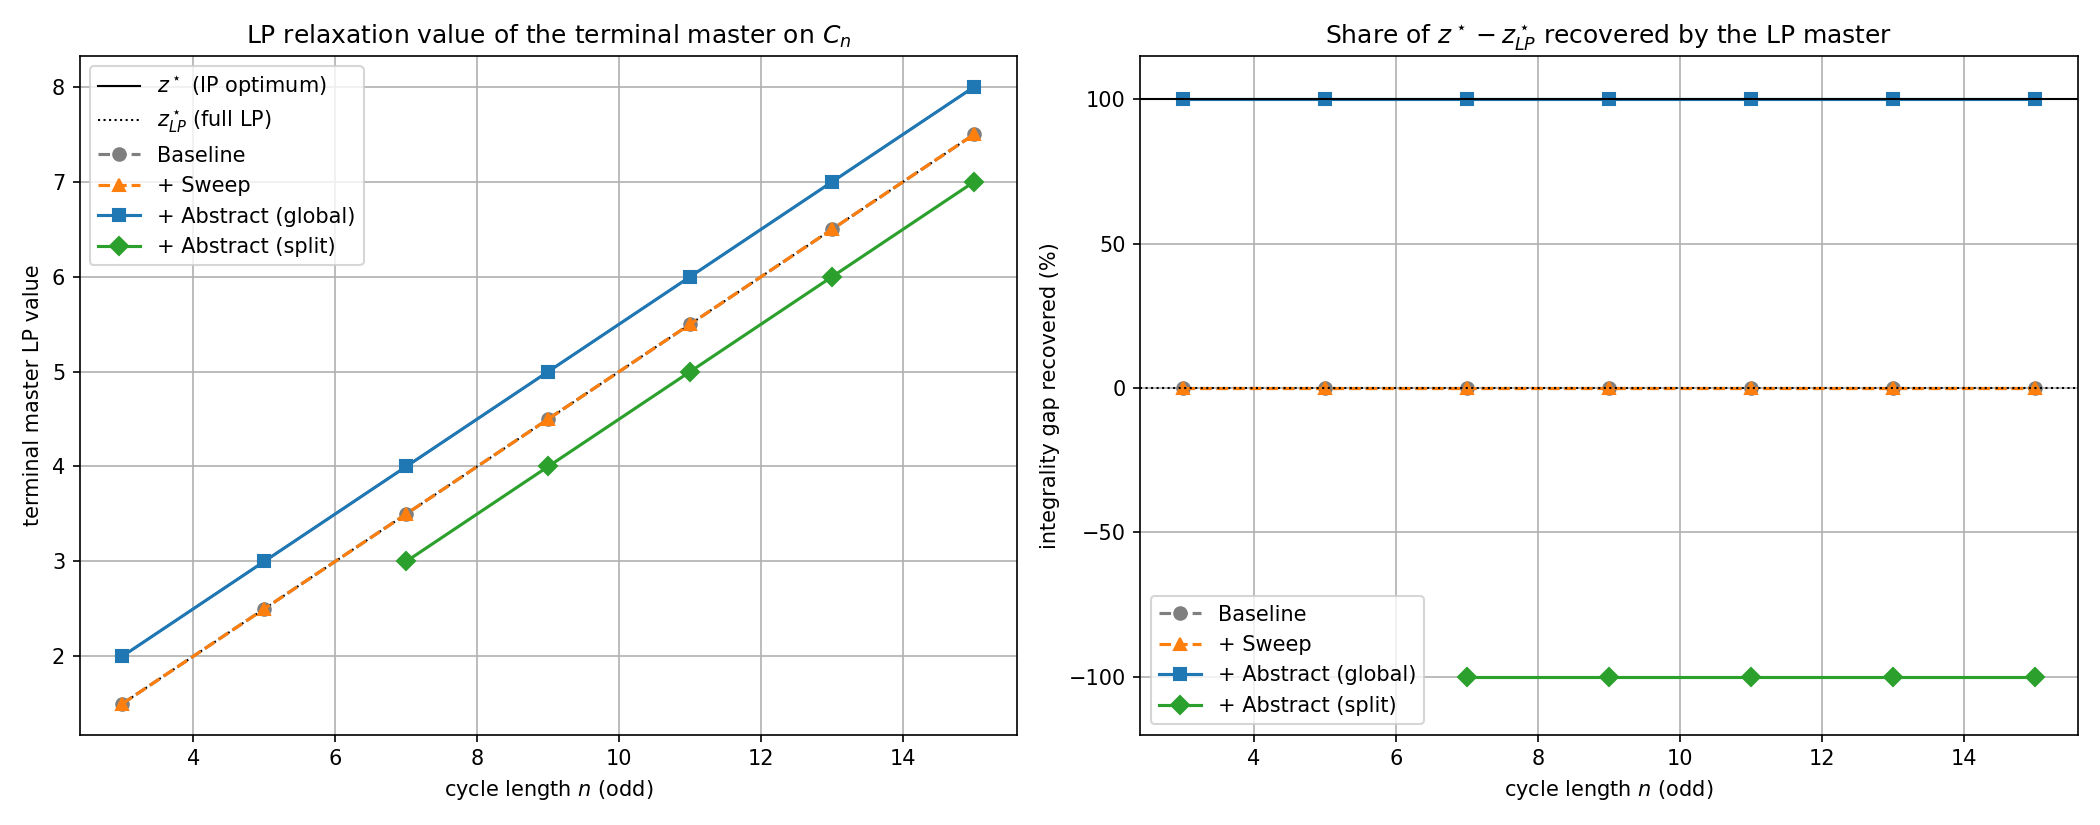
\includegraphics[width=\textwidth]{gap_plot.png}
\caption{Gap recovery on odd cycles $C_n$ (unit weights; $z^\star_{\mathrm{LP}} = n/2$,
$z^\star = (n{+}1)/2$). Left: LP relaxation value of the terminal master.
Right: share of the integrality gap recovered. One aligned abstraction set
covering the cycle recovers the \emph{entire} gap at every size; the split
two-arc clustering produces only mixed (disjunctive) cores and recovers
nothing; the threshold sweep coincides with the baseline because uniform
prices $\bar y_i = \tfrac12$ collapse the sweep to the standard probe.}
\label{fig:gap_recovery}
\end{figure}

\paragraph{Odd cycles: full recovery under aligned aggregation.}
\Cref{fig:gap_recovery} generalizes the $K_3$ counterexample to odd cycles
$C_n$, the canonical family with a persistent vertex-cover gap of
$\tfrac12$. With a single abstraction set covering the cycle, the terminal
LP master attains $z^\star$ at every size---the odd-cycle inequality of
\cref{sec:abstract-cores}, discovered automatically as a rank-$k$
row---while the outer loop shortens from $n{+}1$ iterations (the baseline
must enumerate all $n$ edge cores) to $(n{+}3)/2$. Splitting the same
clauses into two contiguous arcs destroys both effects: every core now
straddles the two sets, only weak normalized surrogates enter the LP, and
the terminal LP value drops \emph{below} $z^\star_{\mathrm{LP}}$ (the run
terminates before accumulating the edge rows the baseline collects).

\paragraph{The aggregation limit is core-guided search.} With one
uniform-weight set covering all soft clauses, the abstract probe asks
``is there a solution falsifying at most $t$ clauses?'' and increments
$t$ on each UNSAT answer---that is, IHS at full aggregation \emph{is} a
core-guided-style linear search over a single cardinality bound (cf.\ the
MSU family of \cref{sec:part1}). The aggregation axis thus interpolates
between the two algorithm families of the duality square
(\cref{sec:unified}): no aggregation is pure IHS, full aggregation is
linear-search core-guided, and the useful regime of abstract cores lies
strictly between.

\begin{table}[htbp]
\centering
\small
\caption{Aggregation alignment on random vertex cover $G(n, 0.2)$
(means over three seeds; CBC/MiniSat prototype). Unit weights give
one aligned global abstraction set; weights drawn from $\{1,2,3\}$ give
three weight-class clusters that cut across the conflict structure.
``Gap rec.''\ is the share of $z^\star - z^\star_{\mathrm{LP}}$ recovered
by the terminal LP master (negative when the terminal master is weaker
than the full ordinary-row LP).}
\label{tab:alignment}
\begin{tabular}{llrrrr}
\toprule
\textbf{Family} & \textbf{Config.} & \textbf{Gap rec.} & \textbf{Iter.} & \textbf{SAT} & \textbf{Time} \\
\midrule
unit, $n{=}25$     & Baseline  & $-7\%$   & $43.0$  & $43.0$  & $1.3$s \\
                   & + Sweep   & $0\%$    & $41.0$  & $89.0$  & $1.3$s \\
                   & + Abstract& $100\%$  & $15.3$  & $15.3$  & $0.4$s \\
\midrule
unit, $n{=}35$     & Baseline  & $0\%$    & $102.0$ & $102.0$ & $3.8$s \\
                   & + Sweep   & $0\%$    & $92.7$  & $202.3$ & $3.5$s \\
                   & + Abstract& $100\%$  & $23.7$  & $23.7$  & $0.7$s \\
\midrule
weighted, $n{=}25$ & Baseline  & $-56\%$  & $43.3$  & $43.3$  & $1.3$s \\
                   & + Sweep   & $-33\%$  & $38.3$  & $81.7$  & $1.2$s \\
                   & + Abstract& $-198\%$ & $40.0$  & $71.7$  & $8.0$s \\
\midrule
weighted, $n{=}35$ & Baseline  & $-2\%$   & $87.7$  & $87.7$  & $3.4$s \\
                   & + Sweep   & $-2\%$   & $82.7$  & $193.3$ & $3.2$s \\
                   & + Abstract& $-1\%$   & $99.0$  & $185.0$ & $36.9$s \\
\bottomrule
\end{tabular}
\end{table}

\paragraph{Random vertex cover: alignment decides the sign of the effect.}
\Cref{tab:alignment} repeats the comparison on random $G(n, 0.2)$ vertex
cover, where the gap arises from many overlapping odd structures rather
than one cycle. Under aligned aggregation (unit weights, one global set)
abstract cores again recover $100\%$ of the gap while cutting iterations
by $3$--$4\times$ and wall time by $5\times$. Under misaligned aggregation
(three weight-class clusters) the effect \emph{reverses}: nearly all cores
are mixed, the LP master gains nothing, SAT calls double, and the
indicator-laden IP master becomes markedly heavier. All configurations
return $z^\star$ in all runs---correctness never depends on the
aggregation---but the profitable regime is exactly the aligned one. This
is the measured face of the crux noted in \cref{sec:abstract-cores}
(``choosing what to aggregate'') and sharpens the motivation for the
dual-informed clustering proposed there: clusters should follow the
conflict structure the master actually prices, not the weight profile
alone. The threshold sweep, for its part, behaves as billed: inert under
uniform prices (odd cycles), and a cheap bound-improvement phase under
heterogeneous prices ($6$--$12\%$ fewer iterations at roughly twice the
SAT calls, time-neutral at prototype scale).
